\documentclass[12pt]{article}
\renewcommand{\baselinestretch}{1.8}
\usepackage{textcomp}
\usepackage{fontenc}
\usepackage{graphicx}
\usepackage{caption} % for Fig. captions
\usepackage{gensymb} % for \degree
\usepackage{placeins} % for \images
\usepackage[margin=1in]{geometry} % to set margins
\usepackage{setspace}
\usepackage{lineno}
%\usepackage{cite}
\usepackage{amssymb} % for math symbols
\usepackage{amsmath} % for aligning equations
\usepackage{natbib}
\usepackage{xr-hyper}
\externaldocument{FLSshort_supp}

\bibliographystyle{..//refs/styles/besjournals.bst}


\linenumbers


\title{Reconciling competing hypotheses regarding flower-leaf sequences in temperate forests for fundamental and global change biology}

\author{D.M. Buonaiuto $^{1,2,a}$, I. Moralles Castilla$^{3}$, E.M. Wolkovich$^{4}$}

%3510 words
\begin{document}
\maketitle
\noindent \emph{Author affiliations:}\\
\noindent $^1$Arnold Arboretum of Harvard University, Boston, Massachusetts, USA\\
$^2$Department of Organismic and Evolutionary Biology, Harvard University, Cambridge, Massachusetts, USA\\
$^3$Department of Life Sciences, University of Alcal\`a CTRA N-II, KM., 33,600, 28802, Alcal\`a de Henares, Spain\\
$^4$Forest \& Conservation Sciences, Faculty of Forestry, University of British Columbia, Vancouver, British Columbia, Canada\\
$^a$Corresponding author: 617.823.0687; dbuonaiuto@g.harvard.edu

\noindent \emph{Keywords:} deciduous forests, flower-leaf sequences, global change, hysteranthy, phenology, phylogeny \\ % 5-8 New Phyto says we should include title words
\emph{Paper type:} Viewpoint\\
 \emph{Counts}: Total word count for the main text: 3370;  5 figures (all in color or 3-4 bw). 40 references (5 extra still appearing). Supporting Information: 4 supplemental figures.\\
\newpage

\section*{Summary}
Phenology is a major component of an organism's fitness. While individual phenological events affect fitness, growing evidence suggests that the relationship between events may be equally or more important. This may explain why deciduous woody plants exhibit considerable variation in the order of reproductive and vegetative events, or flower-leaf sequences (FLSs). Research suggests that FLSs are adaptive, with several competing hypotheses to explain their function. Here, we advance the existing hypotheses with a new framework that accounts for quantitative FLS variation at multiple taxonomic scales using case studies from temperate forests. Our inquiry provides several major insights towards a better understanding FLS variaiton. First, we show that %found?
concurrent support for multiple hypotheses reflects the complicated history of migration and community assembly in the temperate zone. Second, we demonstrate that support for FLS hypotheses is sensitive to how FLSs are defined, with quantative definitions being the most useful for robust hypothesis testing. Finally, we highlight how adopting a quantitative, intra-specific approach generates new avenues for evaluating fitness consequences of FLS variation and provides cascading benefits to improving predictions of how climate change will alter FLSs and thereby re-shape plant communities and ecosystems.

\section*{Introduction}
Phenology, the timing of seasonal life cycle events, allows organisms to synchronize life-history transitions with optimum environmental conditions \citep{Forrest2010}, and is a critical component of ecosystem structure and function \citep{Cleland2007,Piao2007}. Recent work in woody plant phenology has shown that it is not only individual phenological stages that affect these processes, but also the relationships between them \citep{Ettinger2018}.\\

\noindent One phenological relationship that has long received scientific interest \citep[see][]{Robertson1895} and, recently, increased attention in the literature \citep{Savage2019, Gougherty2018} is the flower-leaf phenological sequence (FLS) of deciduous woody plants. In a typical model of plant life-history, vegetative growth precedes reproduction. However, for many species in the forests of Eastern North America (and other temperate regions of the Northern Hemisphere), it is not the green tips of new shoots that mark the commencement of the growing season, but the subtle reds and yellows of their flowers. This flowering-first FLS is common in these forests, and its prevalence suggests that this FLS has adaptive significance \citep{Rathcke_1985}.\\ 

\noindent Understanding this phenological pattern is timely because anthropogenic climate change is altering FLSs. Long-term observations show the number of days between flowering and leafout is increasing as a result of climate change, but the rate of change differs up to five-fold among species (Fig. \ref{fig:climchange}).  If FLSs are indeed an important component of woody plant fitness, this inter-specific variation will exacerbate fitness differences between species, influencing which species will persist under altered climate conditions.\\ 

\noindent Long-term data also highlight high within-species variability in FLSs. Despite recent advances in understanding the physiology and evolution of FLSs \citep{Gougherty2018,Savage2019}, most research has not addressed this variability---potentially slowing progress in predicting how FLS patterns will respond to climate change. While the literature provides some general correlations between flowering and leafing phenology \citep{Lechowicz_1995, Ettinger2018}, there have been few, if any, analyses of higher-resolution patterns \citep{Gougherty2018}. \\

We suggest that characterizing intra-specific variation in FLSs is critical to understanding this important phenological sequence. We propose a new conceptual framework for the study of FLSs built on continuous measures of both inter- and intra-specific FLS variation. This shift will improve our ability to predict how FLS patterns will change in the future, and  may reveal novel avenues to better understand the fundamental biology of this important phenological sequence.\\


\noindent Here we 1) review the hypotheses of the origins of FLSs and their respective predictions, 2) compare the biological basis of the current, inter-specific categorical FLS framework to our proposed intra-specific, quantitative approach 3) test our framework with a detailed case study of long-term phenology records from Harvard Forest in Petersham, MA, and 4) identify avenues for future FLS research.

\section*{Hypotheses for flower-leaf sequences variation and their predictions}
\subsubsection*{ Wind pollination}
\noindent The most prevalent FLS hypothesis suggests that flowering-first is an adaptation for wind-pollination, with leafless flowering allowing for more efficient pollen transfer \citep{Whitehead1969}. The primary evidence for this hypothesis comes from pollen diffusion studies \citep[e.g., particle movement through closed and open canopies,][]{Niklas1985, Milleron2012} and suggests canopy structure encumbers pollen movement. This hypothesis predicts a strong association between FLS and pollination syndrome.
\subsubsection*{Water dynamics}
\noindent Another hypothesis suggests that flowering before leaf development is an adaptation to reduce water stress caused by concurrently maintaining floral hydration and leaf transpiration \citep{Franklin2016}. Observations of flowering in the dry tropics where this FLS pattern is also common confirm that the timing of flowering in these taxa is associated with a water status recovery due to leaf drop \citep{Borchert1983,Reich1984}, and recent analysis of temperate flora has also yielded support for this hypothesis despite that fact that temperate forests are rarely water-limited during the spring flushing season \citep{Gougherty2018}. This hypothesis predicts a strong relationship between FLS and metrics of hydraulic demand.
 
\subsubsection*{Early flowering}
\noindent A third possibility is that the flowering-first FLS is a physiological byproduct of selection for early flowering \citep{Primack1987}. Here, there is no functional advantage to a species flowering before or after leafing; all that matters is its absolute flowering time. \citet{Primack1987} notes that flowering-first species tend to also have large seed mass and lack primary seed dormancy for germination, traits associated with early flowering in general. This raises the possibility that this FLS may simply be one component of a larger suite of early flowering traits. Recent work from \citet{Savage2019} demonstrated that spring flower phenology is less constrained by prior phenological events than leaf phenology, which would allow selection to drive flowering into the early season, producing the the flowering-first FLS. Given this hypothesis, we would expect a strong relationship between a flowering-first FLS and early flowering in general.

\subsubsection*{Phylogenetics} 
\noindent Finally, it is also possible that FLSs are highly conserved traits for which FLS variation reflects macro-evolutionary relationships among taxa. If this is the case, we would expect to see a strong phylogenetic signal for FLS variation as was reported in a recent analysis by \citet{Gougherty2018}. A strong phylogenetic pattern to FLS variation does not proclude any of the adaptive hypotheses presented above, as  many different evolutionary processes can yield comparable phylogenetic signals \citep{Revell2008}. \\

\noindent While decades of inquiry have advanced each of these hypotheses independently, there is no clear consensus regarding their comparative merits. Most of the previous studies on FLSs have not compared hypotheses, and those that did have generally found support for multiple hypotheses \citep[see][]{Bolmgren2003,Gougherty2018}. There is no expectation that the FLS hypotheses must be mutually exclusive. Indeed, understanding the relative importance of each one and the relationships between them may provide the most useful path forward, if they can be robustly compared.\\


\noindent We argue that a satisfying reconciliation of these hypotheses is possible with a shift to a new conceptual framework for the study of FLSs. Under the current framework, FLSs are described qualitatively, and defined at the species level. We suggest that quantitative, intra-specific measures of FLS are more compatible with the biological processes underlying the very FLS variation that research aims to understand. Below we present an overview of the classic approach to describing FLSs and highlight some of the challenges that can arise when using it. \\

\section*{The current flower-leaf sequence framework}
\subsection*{Describing FLSs}
\noindent  The current framework describes three main FLS categories: flowers before leaves (hysteranthy, proteranthy, precocious flowering); flowers with leaves (synanthy); and flowers after leaves (seranthy) \citep{Lamont2011, Heinig1899}. Some data sources \citep[e.g.][]{Burns1990,Barnes2004} include additional categories: ``flowers before/with leaves" and ``flowers with/after leaves", but it is unclear whether these categories describe intermediate FLS patterns or FLS variability in these species. While these categories are conceptually reasonable, applying them to real phenological sequences is not always straightforward.\\

\noindent Both reproductive and vegetative phenological sequences consist of multiple sub-stages, and this introduces significant ambiguity into how we interpret qualitative FLS descriptions. Consider a species with the following FLS:\\

\begin{center}
\textbf{flower budburst}$\rightarrow$ \textbf{leaf budburst}$\rightarrow$ \textbf{first flowers open} $\rightarrow$ \textbf{leafout} $\rightarrow$ \textbf{peak flowering} $\rightarrow$ \textbf{end of leaf expansion} \\
\end{center}

\noindent Observers could justifiably classify this species as: 1) Hysteranthous because flower budburst proceeds leaf budburst, 2) Synanthous because flowers open during the budburst-leafout inter-phase, 3) Seranthous because peak flowering occurs after leafout. This problem extends beyond this simple example to real datasets, \citep[e.g.][]{OKeefe2015} where the same ambiguities exist (Fig \ref{fig:HFmeans}). Not surprisingly then, different sources may classify the same species differently. We compared species-level FLS descriptions in two of the most comprehensive records of FLS, \underline{Michigan Trees} and its companion volume \underline{Michigan Shrubs and Vines} (MTSV) \citep{Barnes2004,Barnes2016} with \underline{The USFS Silvics Manual Volume II} \citep{Burns1990}. Of the 49 overlapping species, 30\% were classified differently. Such different classifications could reflect interesting temporal or geographic variability in FLSs, but---given current definitions---they could equally be the product of observer classification decisions.\\

\noindent Categorization can often introduce biases in analyses \citep{Royston2006}. In the case of FLSs, the hypotheses themselves may suggest different boundaries than the ones prescribed by the traditional framework. The wind pollination hypothesis hinges on the fact that leaves create a substantial physical disruption to pollen transfer, a premise that would not necessarily be true for the early stages of leaf expansion when tiny leaf primordia would have little impact on environmental structure. Rather, trees that flower during the early stages of leaf expansion should gain similar advantage to those who complete their flowering before any leaf activity. Alternatively, because transpiration intensifies as soon as leaves begin to expand \citep{%Breda1996,
Wang2018}, the water dynamics hypothesis asserts there should a cost to maintaining floral structures during any stage of leaf activity. Here, only species where flowering occurs before any leaf expansion should gain a hydraulic advantage.\\ 

\noindent Given the differences in biological processes underlying these hypotheses, statistical relationships between FLS and traits will fluctuate depending on where categorical boundaries are drawn. For the example presented above, we would expect to see the strongest signal of the wind-pollination hypothesis when the category of hysteranthy includes species that flower before and with early leaf development. The strongest signal for the water dynamics hypothesis should occur when the hysteranthous classification is restricted to only species that flower before any leaf activity. If these hypotheses require different categorization schemes to accurately capture the underlying biology, it becomes very difficult to compare hypotheses in the same modeling framework.\\

\noindent For both the MTSV and USFS data sets, we found that the strength of associations between FLS and trait predictors as well as the phylogenetic signal are highly sensitive to how FLSs were defined (Fig: \ref{fig:muplots.USMT}, e.g. pollination syndrome, Fig: \ref{fig:Dstat}). For both datasets, we applied two alternative FLS categorizations; physiological hysteranthy, which allowed for no overlap between floral and leaf phenophases, and functional hysteranthy, which allowed for a degree of overlap. These alternate categorization boundaries re-shuffled the species included in each classification, affecting both the trait distributions within each category and the phylogenetic patterning across the tree (Fig. \ref{fig:phylogeny}).\\ 
 
\noindent These findings suggest that a new approach that relaxes the assumptions of the categorical framework is needed to fairly evaluate FLS hypotheses. Given that these hypotheses all aim to explain FLS variation, the most useful definitions of FLS should follow from FLS variability in nature. Below we consider two major assumptions about FLS variation in the current framework and how they compare to the observed phenological patterns in natural systems.\\

\subsection*{Inter- and intra- specific variation in the current framework}
\noindent In current framework species are classified based on sequence alone. The duration of and time between phases, however, also matters \citep{Inouye2019}. When considering measures of time, FLSs of species within each category can be quite different (Fig. \ref{fig:vizzy}a), suggesting much greater diversity in FLS patterns in a given forest community than provided by the three categories of the current framework. This substantial inter-specific variation could be the fingerprint of selection on FLSs.\\ 

\noindent Under the current framework, FLS categories are assigned at the species level. However, the time between flowering and leaf activity can vary by as much as several weeks between individuals and years, and in some species the sequence itself can regularly switch across years (as seen in the long-term phenology records from  Harvard Forest \citep{OKeefe2015}, Fig. \ref{fig:vizzy}b). Intra-specific variation in FLSs is rarely quantified, yet the magnitude of variation at this level suggests that considering FLSs at finer taxonomic resolution--i.e. intra-specifically--could help clarify the mechanisms underlying inter-specific differences.\\

\section*{A new framework for flower-leaf sequences} 

\noindent Alternative approaches to estimating FLSs could increase the precision of FLS descriptions and capture important biological variation, which could then be leveraged to better understand this phenological syndrome. A shift from categorical, species-level descriptions of FLS to continuous individual-level quantification---i.e. reporting the number of days between specific phenophases---eliminates categorization bias, reduces the noise associated with unmeasured variation, and offers novel avenues for fine-tuning FLS hypotheses.\\ 

\noindent  Quantitative measures of FLSs across multiple taxonomic scales should improve FLS-trait association models like the ones presented above by allowing researchers to explicitly incorporate the multiple levels of FLS variation into such models (i.e. through hierarchical modeling). Quantitative measures of phenology \citep[e.g. the BBCH scale,][]{Finn2007} also standardize data across time and space, observer, and analyst. Adopting these alternative measurements in the study of phenological sequences would facilitate comparing FLS patterns across larger temporal, geographic, and taxonomic scales, giving researchers more power to accurately address questions about FLS variation.\\

\noindent Additionally, an intra-specific FLS framework augments the existing FLS hypotheses and generates new, testable predictions. When considering the FLS hypotheses at multiple taxonomic scales one might a) find a strong inter-specific signal but only noise in the variation within species b) find a strong intra-specific signal but not marked differences across species, or c) find congruence at the species and intra-species levels. Resulting patterns may thus be informative about the evolutionary processes behind FLS variation--e.g. phylogenetic or physiological constraints  vs. adaptation as a response to selection \emph{Nacho, this is pretty much your idea, do you think we need to clarify exactly how these patterns would be interpreted? Do you have any ideas how to elaborate or clarify this idea?}.\\

\noindent Finally, it follows from the FLS hypotheses that variation in FLS should influence performance. This prediction may be difficult to evaluate at the species-level because species evolve a suite of traits for any function \citep{Davies2019}, and unmeasured traits may compensate for FLS variation. Leveraging intra-specific variation could provide a more tractable way for researchers to study FLS-performance relationships, allowing researchers to move beyond simple FLS-trait correlation analyses, and towards evaluating the performance consequences of FLS variation. Such studies could help anticipate the fitness effects of changing FLS patterns with climate change.\\

\section*{Testing the new framework}

% EMW (2Mar): Recommend we avoid 'classic' -- sounds like we're trying to do a takedown
To test our proposed framework, we modeled the associations between FLS and traits related to the FLS hypotheses using both the current categorical FLS framework and our proposed quantitative one, using long-term phenological records for woody species at Harvard Forest \citep{OKeefe2015}. With the categorical approach, we found strongest support for the early flowering hypothesis, some support for the wind pollination hypothesis and poor support for the water dynamics hypothesis, with no substantial interactions between predictors and a strong phylogenetic structure to FLS variation (Fig. \ref{fig:muplots.HF}, Fig.  \ref{fig:Dstat} panel f.). These results are qualitatively similar to models from two other large categorical FLS datasets (Fig. \ref{fig:muplots.USMT}). \\

\noindent The quantitative version of the model paints a more complex picture of the function of FLSs, highlighting key biological insights obscured by categorization. As in the categorical model, we found strong effects of flowering time, pollination syndrome and phylogeny on FLS variation (Fig. \ref{fig:muplots.HF}, Fig. \ref{fig:Dstat}). However, in the quantitative model we also detected a signal for the water dynamics hypothesis. %not exactly sure how to explain this result
Most significantly, in this model we identified strong interactions between predictors. While early flowering is associated with hysteranthy in all species, this effect was even more pronounced in wind-pollinated taxa. (Fig. \ref{fig:muplots.HF}). Further, we also found that water dynamics were associated with increased time between flowering and leafing in biotically-pollinated taxa but not wind-pollinated taxa (Fig. \ref{fig:apcs}). \\ 

\noindent These systematic differences between pollination syndromes are informative. While a relationship between any species' hydraulic demand and their FLS in the temperate zone where water tends to be abundant in the spring \citep{Polgar2011} may seem surprising, many of the biotically-pollinated species of the temperature forests trace their bio-geographic origins to the same dry-deciduous tropical regions \citep{Daubenmire1972} in which the water dynamics hypothesis originated \citep{Janzen1967,Franklin2016}. In particular, many biotically-pollinated, hysteranthous species in the temperate zone are geographic outliers from largely tropical clades (e.g. \textit{Fabaceae}, \textit{Lauraceae}, \textit{Annonaceae}). Thus, these results lead to the hypothsis that, for these taxa, hysteranthy developed in a warmer, drier selection environment and has been maintained in the temperate zone because of high phylogenetic conservatism, or because it has been re-purposed for a different function. 
This migration-conservatism hypothesis has been invoked to explain community phenology patterns in other forest systems \citep[i.e. general flowering in dipterocarps,][]{Kurten2018}. While this link is only speculative for the occurance of biotically-pollinated hysteranthous species in the temperate zone, the bio-geography behind our findings suggests a more complex story of convergent evolution, migration history, and community assembly in hysteranthous flowering than can be encompassed by any single FLS hypothesis.\\

\noindent Our findings suggest that the tendency for previous studies to find support for multiple hypotheses \citep{Bolmgren2003,Gougherty2018,Savage2019} is consistent with the biological processes that shape FLSs. Using available data, we have demonstrated the advantages of a new conceptual framework for the study of FLSs based on quantitative measures of individual variation in FLS patterns. Using these methods, we found that, in accordance with previous work, flowering time and pollination syndrome are important drivers of hysteranthy \citep{Gougherty2018}. We also found support for the water dynamics hypothesis in the evolutionary history of biotically-pollinated taxa, and identified several new, testable hypotheses regarding the biological nuances of FLSs. Together, these results provide a more comprehensive picture of our understanding of this phenological trait currently, and pathways for further research. Below we highlight four characteristics of FLS that we suggest could be incorporated into future research that utilizes this new framework to improve our fundamental knowledge about this important life-history trait and better predict how alterations to FLSs will impact species in an era of global change.\\
\section*{Future directions:}
\subsubsection*{Multiple hypotheses explain FLSs}
\noindent Our results underscore other lines of evidence that show multiple hypotheses should be the starting point for future FLS research. While there is certainly value to broad taxonomic studies, and future large-scale analyses should continue, the consistent support for multiple hypotheses shows there are limits to the utility of these kinds of studies. We suggest future studies explore the evolutionary dynamics of hysteranthy with a more mechanistic approach, which may mean utilizing a more taxonomically-restricted focus. A better understanding about the mechanisms leading to FLS variation may result from pattern deconstruction \citep[i.e. grouping of species according to trait commonalities or their geographic or phylogenetic distributions,][]{Terribile2009} For example, as wind-pollination efficiency is not driving hysteranthous flowering among biotically-pollinated taxa, considering this group of species alone rules out one major FLS hypothesis and would allow for a better evaluation of alternative hypotheses.

\subsubsection*{FLS, performance and fitness}
Even with focused work on sub-groupings of species, inter-specific trait-association models may provide more limited advances than other approaches. As in most other areas of plant biology examining traits, research is hampered by the difficulty of knowing which are the ``right'' traits \citep{Violle2007}. For example, we used minimum precipitation across a species' range, one of the only available quantitative drought metrics at the scale of large inter-specific models, to represent the water dynamics hypothesis, but we have little data to evaluate if this is a good proxy for hydraulic demand or drought tolerance. \\

% EMWJan7: Nice opening here.
\noindent While trait associations point to past selection, fitness is the driver of trait evolution, and at the core of each FLS hypothesis is a fitness prediction. By utilizing intra-specific comparisons and continuous measurements of FLS, we can move beyond trait associations and test the performance consequences of FLS variation. As we discussed above, variability in hysteranthy should lead to variability in performance outcomes at the intra-specific level. For example, the wind pollination hypothesis predicts that years with increased time between flowering and leafing should correlate with more pollination success. The water dynamics hypothesis suggests hysteranthous populations with a consistently larger time between flowering and leafing should better tolerate drought. These predictions could be directly assessed through well-designed experiments and field studies, providing a new avenue to test the existing hypotheses and better understand how variability in performance may or may not ultimately translate into differential fitness as FLSs continue to shift due to climate change.

\subsubsection*{FLS and physiology} 
\noindent Decades of research shows that both floral and vegetative phenological events are cued by temperature and photoperiod \citep{Forrest2010}, suggesting they are under shared genetic and physiological control. But to yield the FLS variation seen in nature, there is likely systematic differences in reproductive and vegetative phenological responses to the environment. Researchers can use intra-specific variation in FLS to identify which cues dominate each phenological process and better understand the underlying genetic and physiological constraints that structure phenological sequences.

\subsubsection*{Linking individual phenophases and sequences}
\noindent While much of research on the evolution of plant phenology focuses on specific phenophases  \citep[e.g.][]{Savage2013,OLLERTON_1992}, in this paper, we examined the evolutionary drivers of a phenological sequence. With growing evidence that adaptation drives both the absolute timing of individual phenophases and the relative timing between them we must continue to develop analytical tools that improve our understanding of the drivers of phenological events as part of a phenological syndrome, rather than as discrete, separate events. 
Our treatment of FLSs here is a small part of this work, but understanding how selection shapes phenology both throughout the whole growing season and across years remains an exciting frontier for the study of phenology \citep{Wolkovich2014b}.

\subsection*{Conclusion:} 
\noindent Our proposed framework provides a path to understanding the drivers of FLSs in woody plants. Through examining FLS variation in more targeted taxonomic assemblages and using quantitative data with mechanistic metrics, we can refine the existing FLS hypotheses and better comprehend the causes and consequences of FLS variation at multiple taxonomic scales. This is an essential step towards a more complete understanding of the fundamental biology of temperate woody plants, and for predicting the fate of these species as global climate continues to change.

\section*{Aknowledgements}
\begin{itemize}
\item T.J. Davies
\item J.J Grossman
\end{itemize}

\section*{Author contributions}

% EMW (2Mar): Still some ref issues to clean up.
\bibliography{..//refs/hyst_outline.bib}

\newpage
\section*{Supplimental Information}
Figure S1: Effect-size summary plots of FLS predictors for the MTSV and USFS case studies. \\
Figure S2: Flower-leaf sequences of species at Harvard Forest 1990-2005.\\
Figure S3: Phylogenetic signals for FLS variation.\\
Figure S4: Visualization of FLS patterning across the phylogeny for the MTSV and USFS case studies.\\
Methods S1: Methods for: FLS and climate change modeling, modeling FLS variation in MTSV and USFS data, modeling FLS variation in the HF data, and calculating the phylogentic signals in FLS variation.
\newpage
\section*{Figures}

\begin{figure}[h!]
    \centering
 %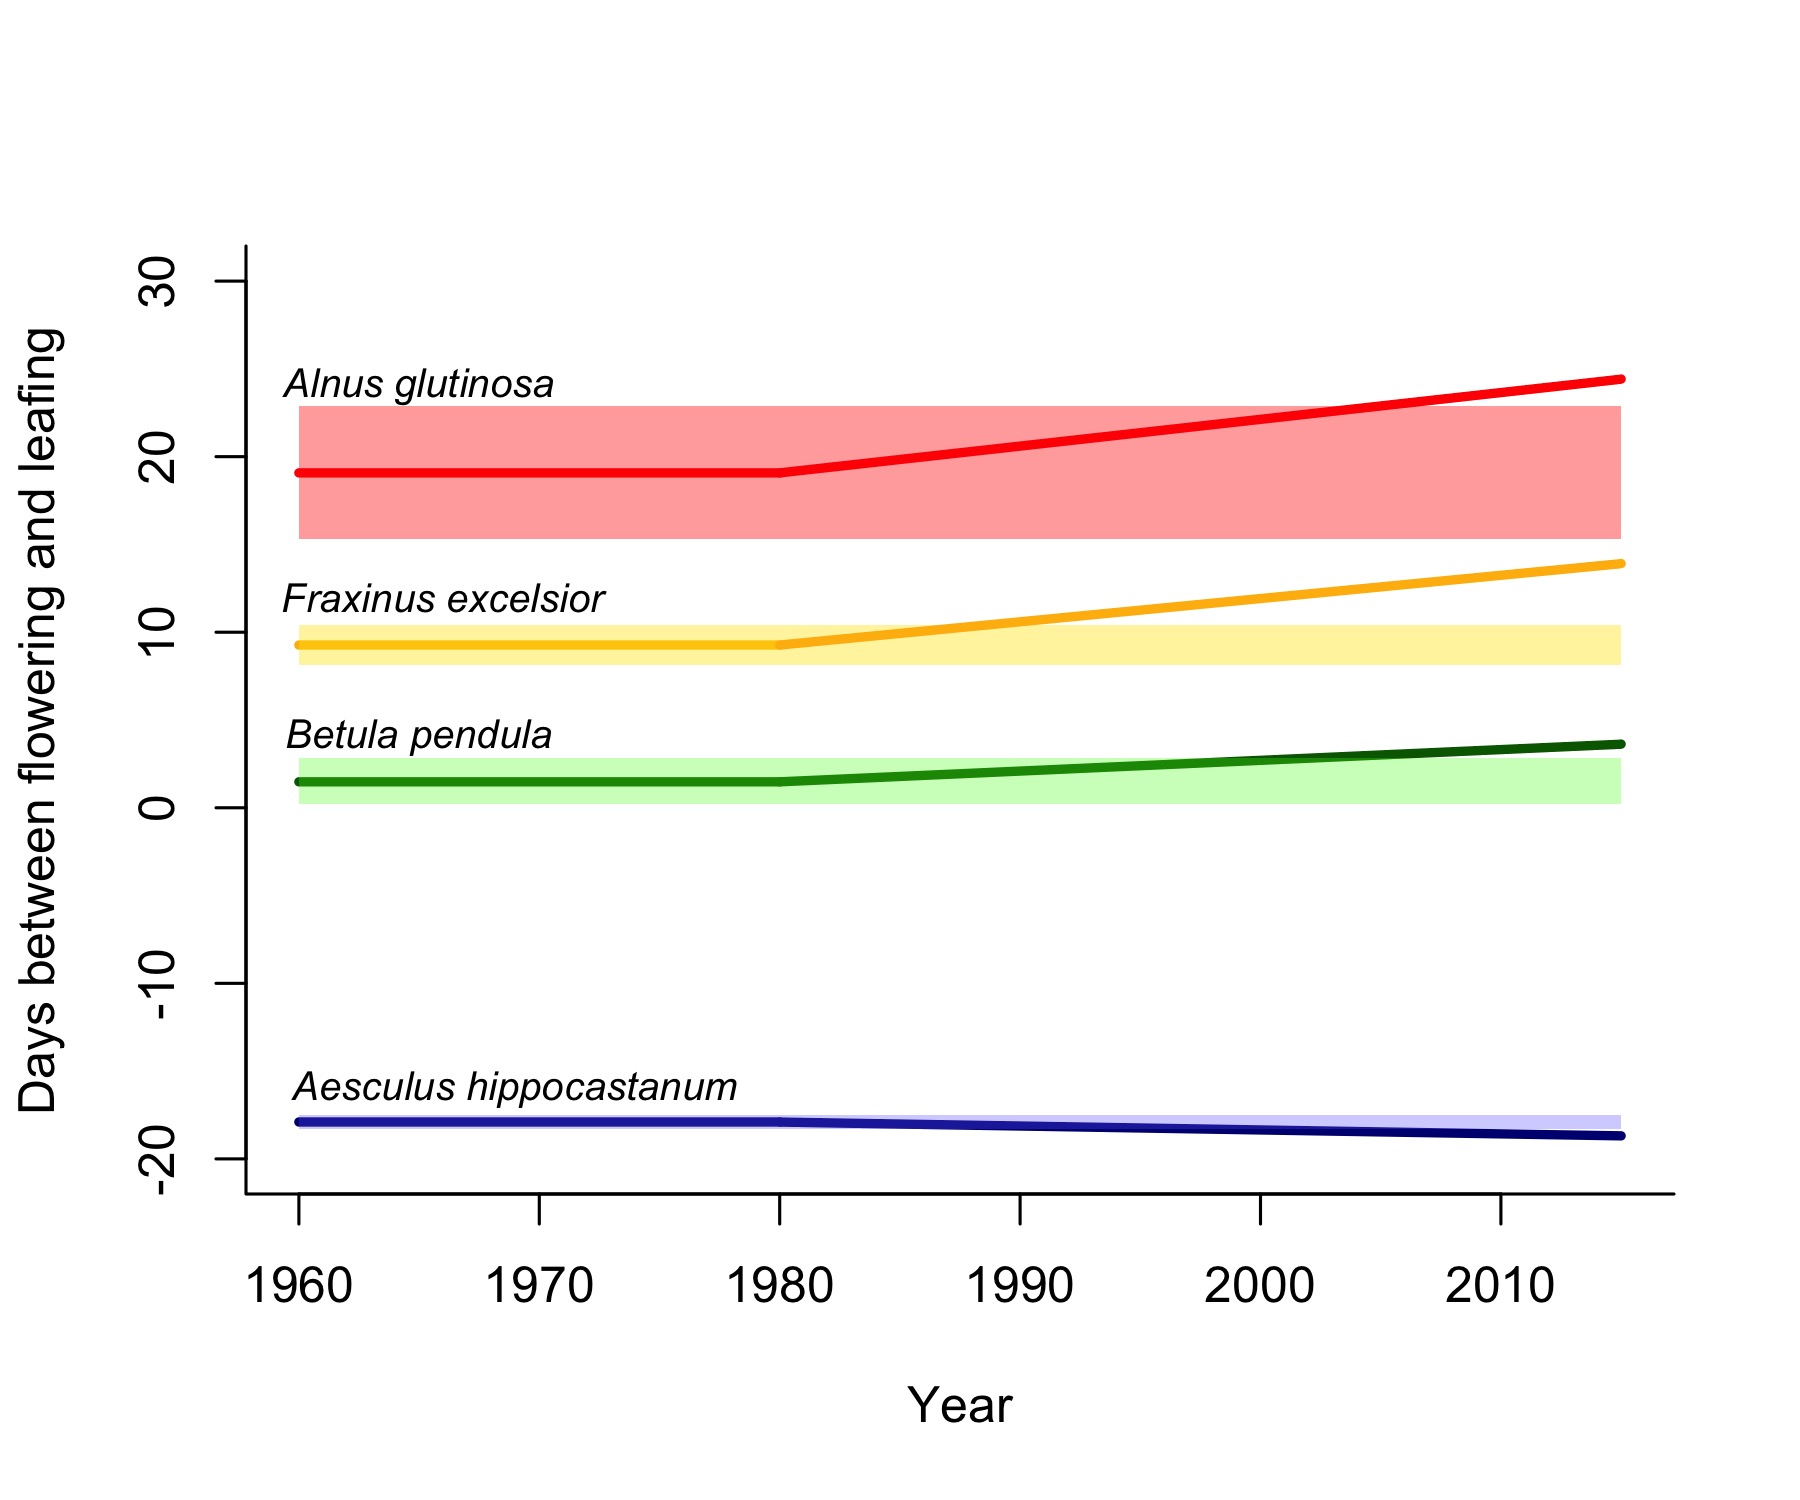
\includegraphics[width=\textwidth]{..//PEP725/FLS_climate_change.jpeg} 
    \caption{\textbf{Flower-leaf sequences (FLSs) across Europe for four tree species from 1960 to 2015 suggests climate change has generally increased the time between flowering and leafing}, but the direction and rate of change differs across species, which may exacerbate fitness differences within forest communities. To detect the effect of climate change on average FLS, we used models that allow for shifts in FLS after 1980. Lines represent the mean trend in FLS per species, and the highlighted regions indicate historic range of FLS variability (95\% credible intervals of the pre-1980 average) from the PEP725 database \citep{PEP725}.}
    \label{fig:climchange}
\end{figure}
 
 \begin{figure}[h!]
        \centering
    %      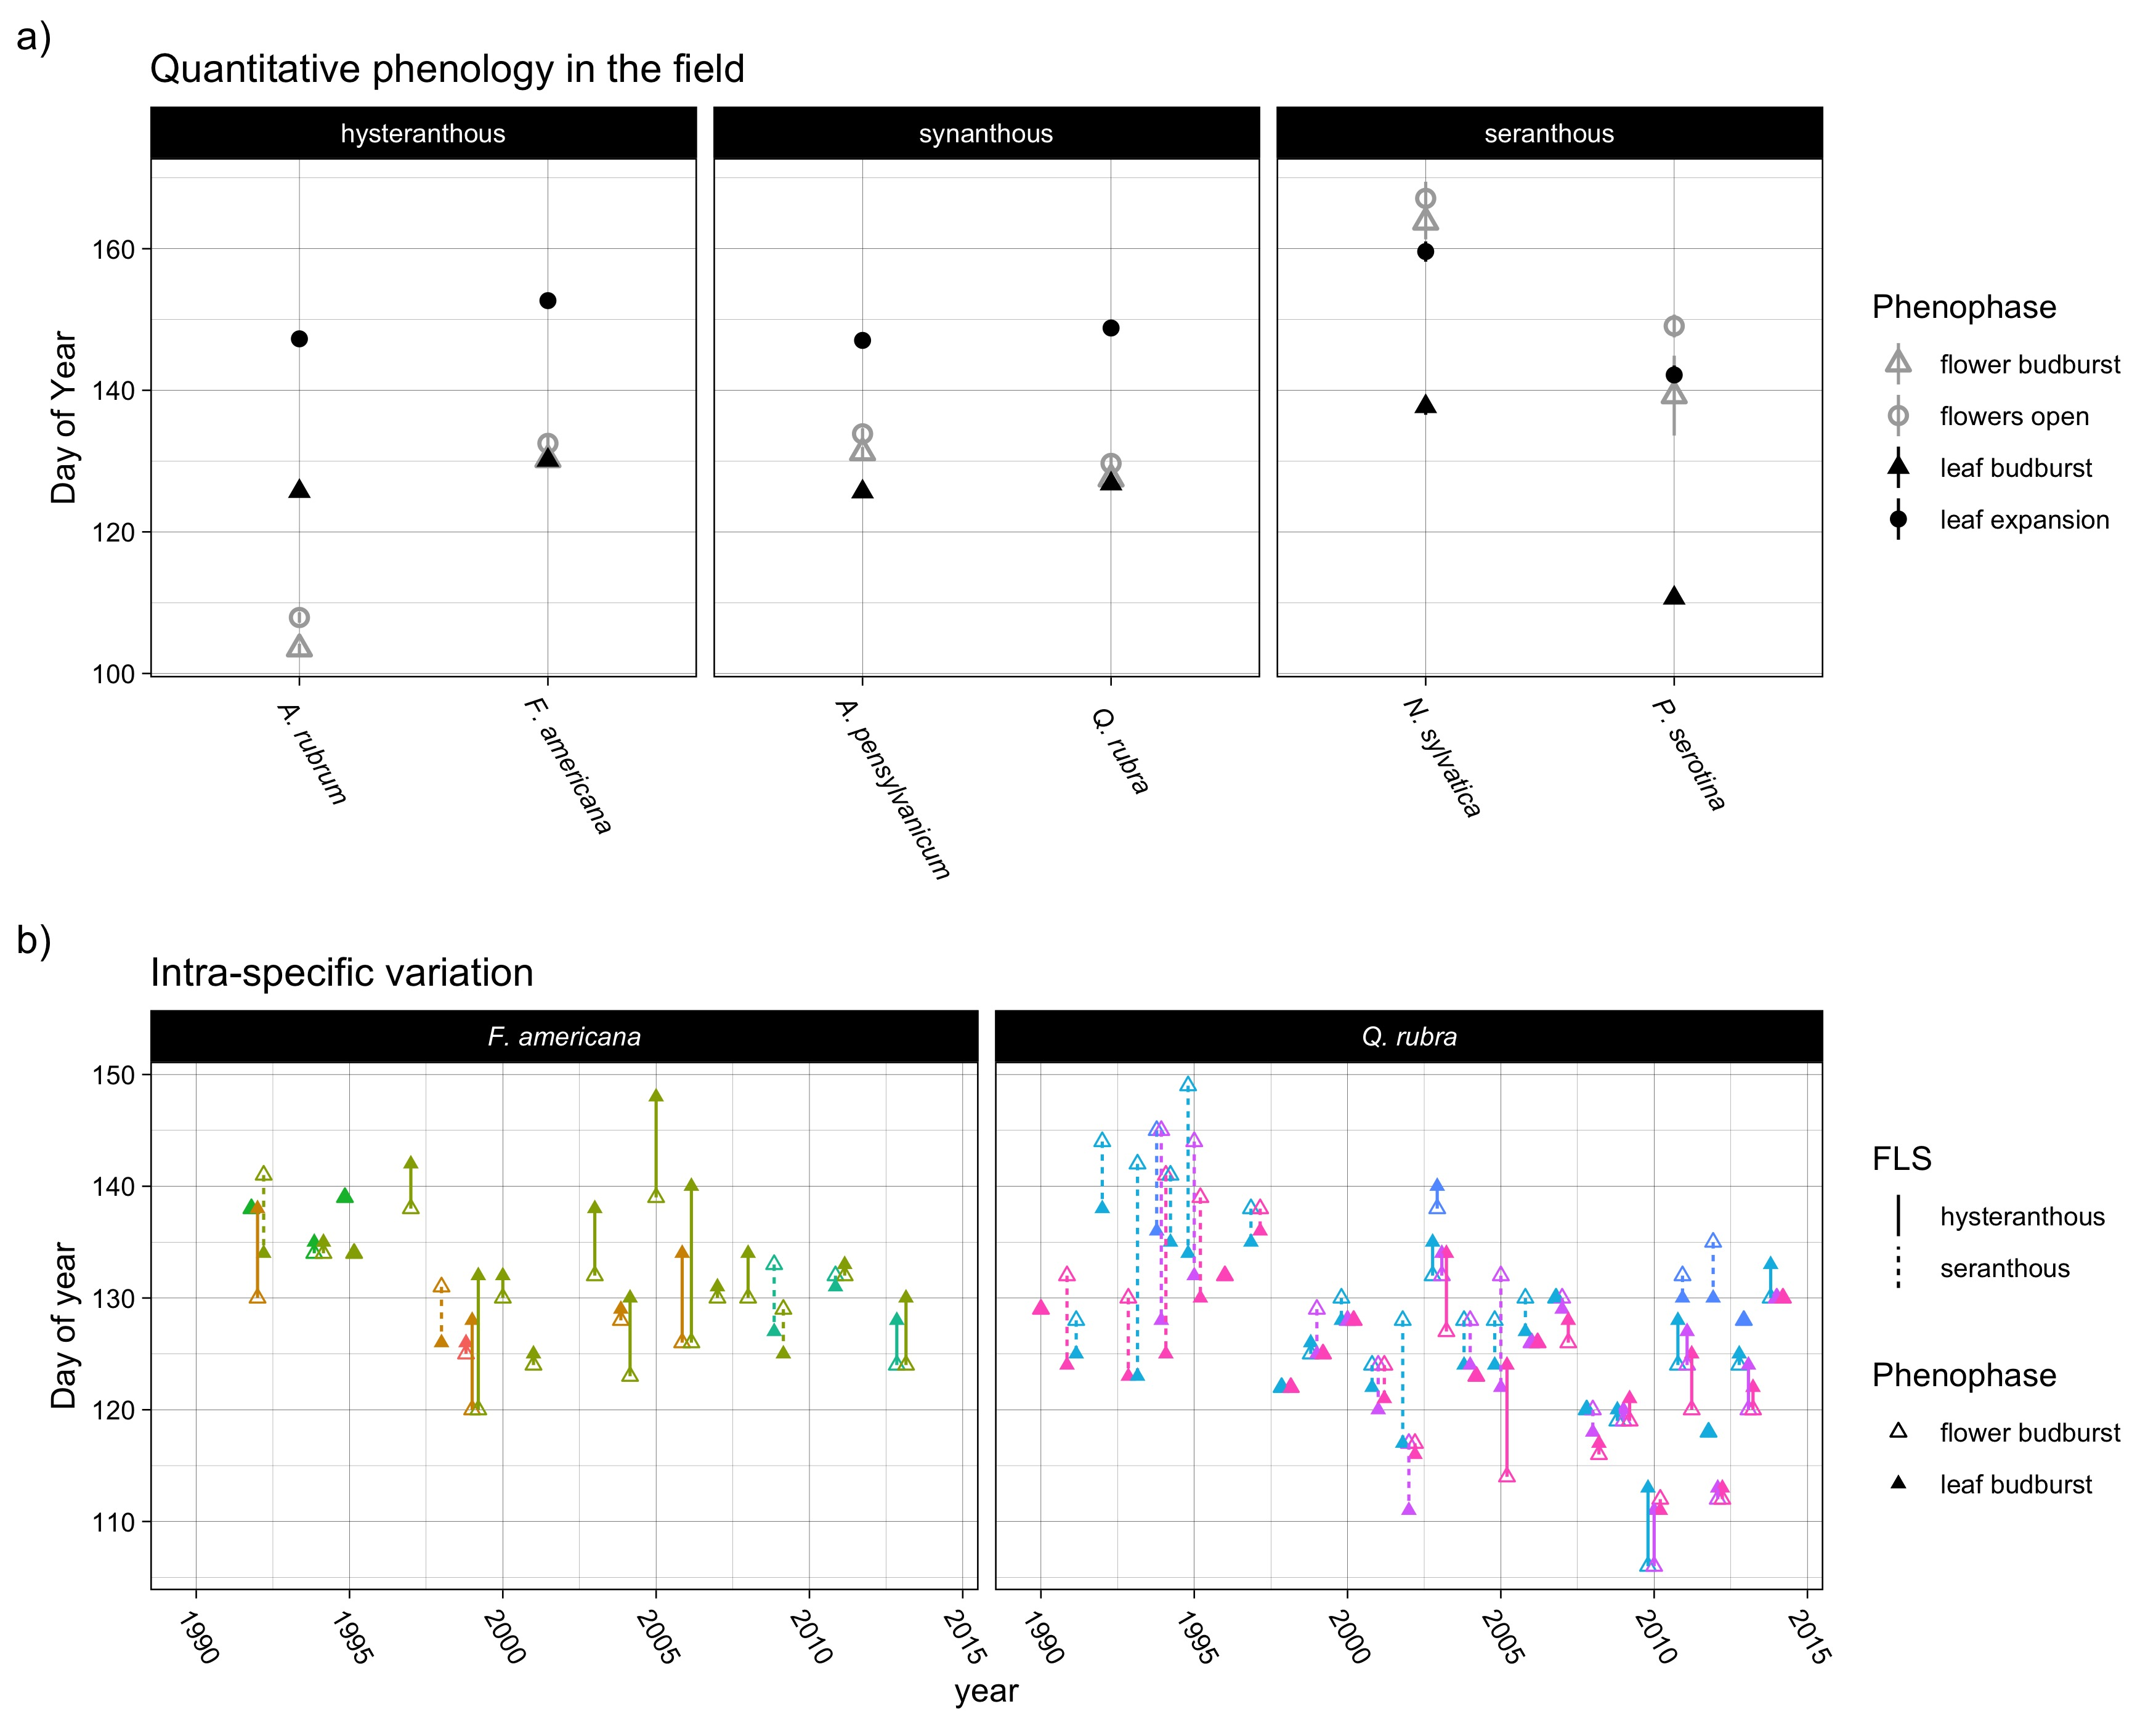
\includegraphics[width=\textwidth]{..//HarvardForest/FLS_viz.jpeg}
          \caption{\textbf{The shift from categorical/inter-specific descriptions to quantitative/intra-specific measures of flower-leaf sequences (FLSs) reveals substantial variation.} Under the current framework, species are assigned to FLS categories by the order of phenophases alone. However, observations from Harvard Forest in Petersham, MA demonstrate that measuring the time between phenophases reveals substantial differences among species within each category \textbf{(a)}. These records also show that below the species level \textbf{(b)}, the time between flowering and leaf activity can vary by as much as several weeks for an individual across years and, in some species, an individual's sequence itself regularly switches across time. This inter- and intra- specific variation is key understanding the function of FLS variation in deciduous, woody plants.}
        \label{fig:vizzy}
    \end{figure}

\pagebreak  

 \begin{figure}[h!]
        \centering
    %      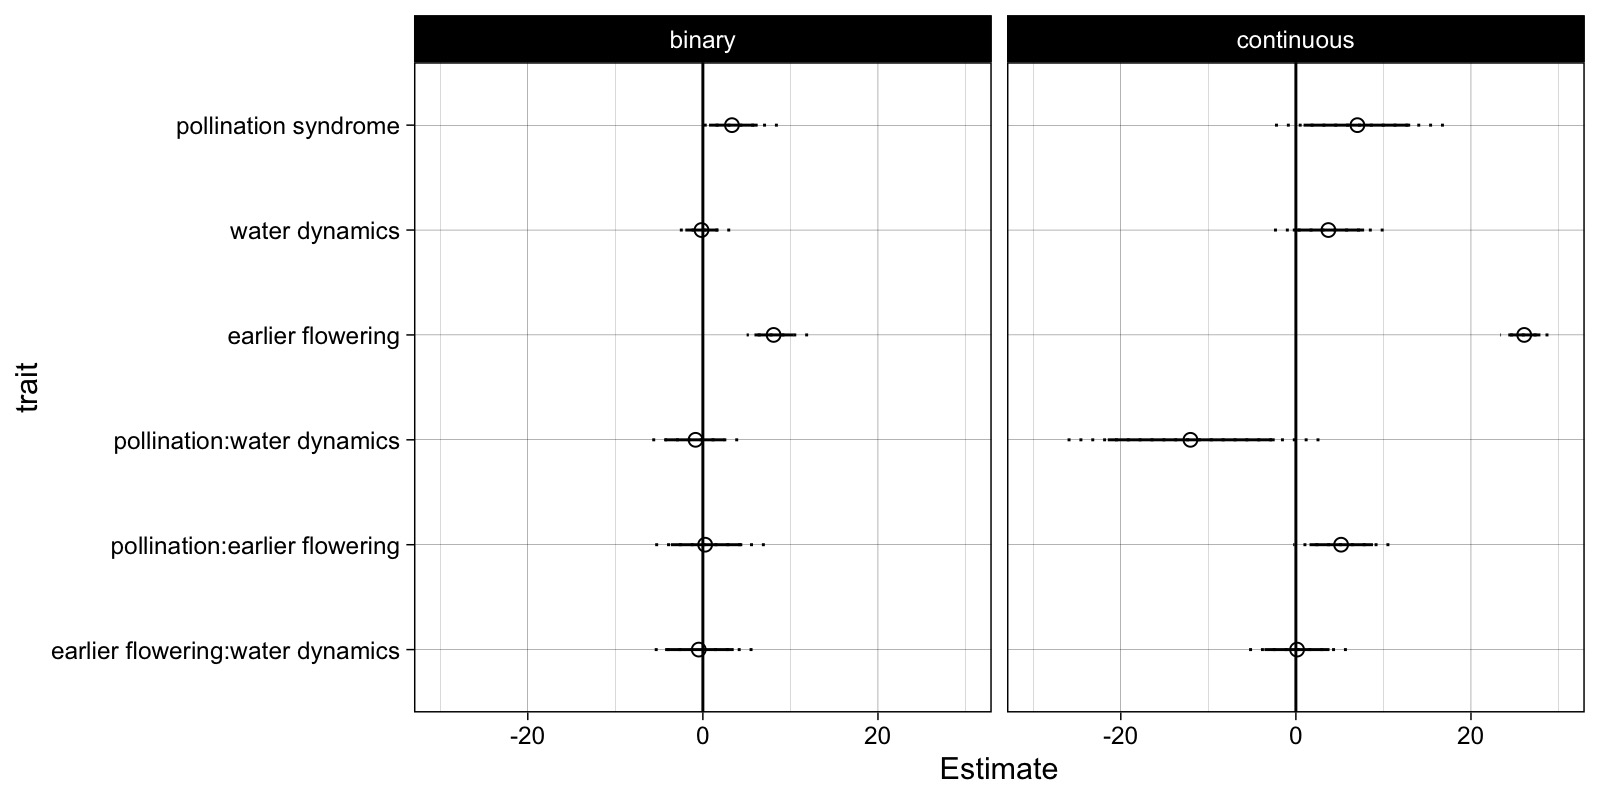
\includegraphics[width=\textwidth]{..//HF.jpeg}
          \caption{\textbf{Mean estimates of the effects of flower-leaf sequence (FLS) predictors on the timing between flowering and leaf expansion for individual woody plants at Harvard Forest between 1990-2015 reveal important differences between categorical and quantitative frameworks of FLS.}  With the categorical approach, there is a strong effect of flowering time and pollination syndrome on FLS variability, with no detectable effect of water dynamics or interactions between the predictors. However, with quantitative measures of FLS, we find increased support for the water dynamics hypothesis, and strong interactions between pollination syndrome and both flowering time and water dynamics. This interactions suggest multiple drivers of FLS variability in the temperate zone.  Both models use a Bayesian, phylogenetic mixed modeling approach with standardized predictors to allow for comparisons between them. Symbols represent mean estimated effect of each predictor, with solid and dotted lines representing 50 and 95\% credible intervals respectively.}  
        \label{fig:muplots.HF}
    \end{figure}    

    

 \begin{figure}[h!] 
        \centering
 %         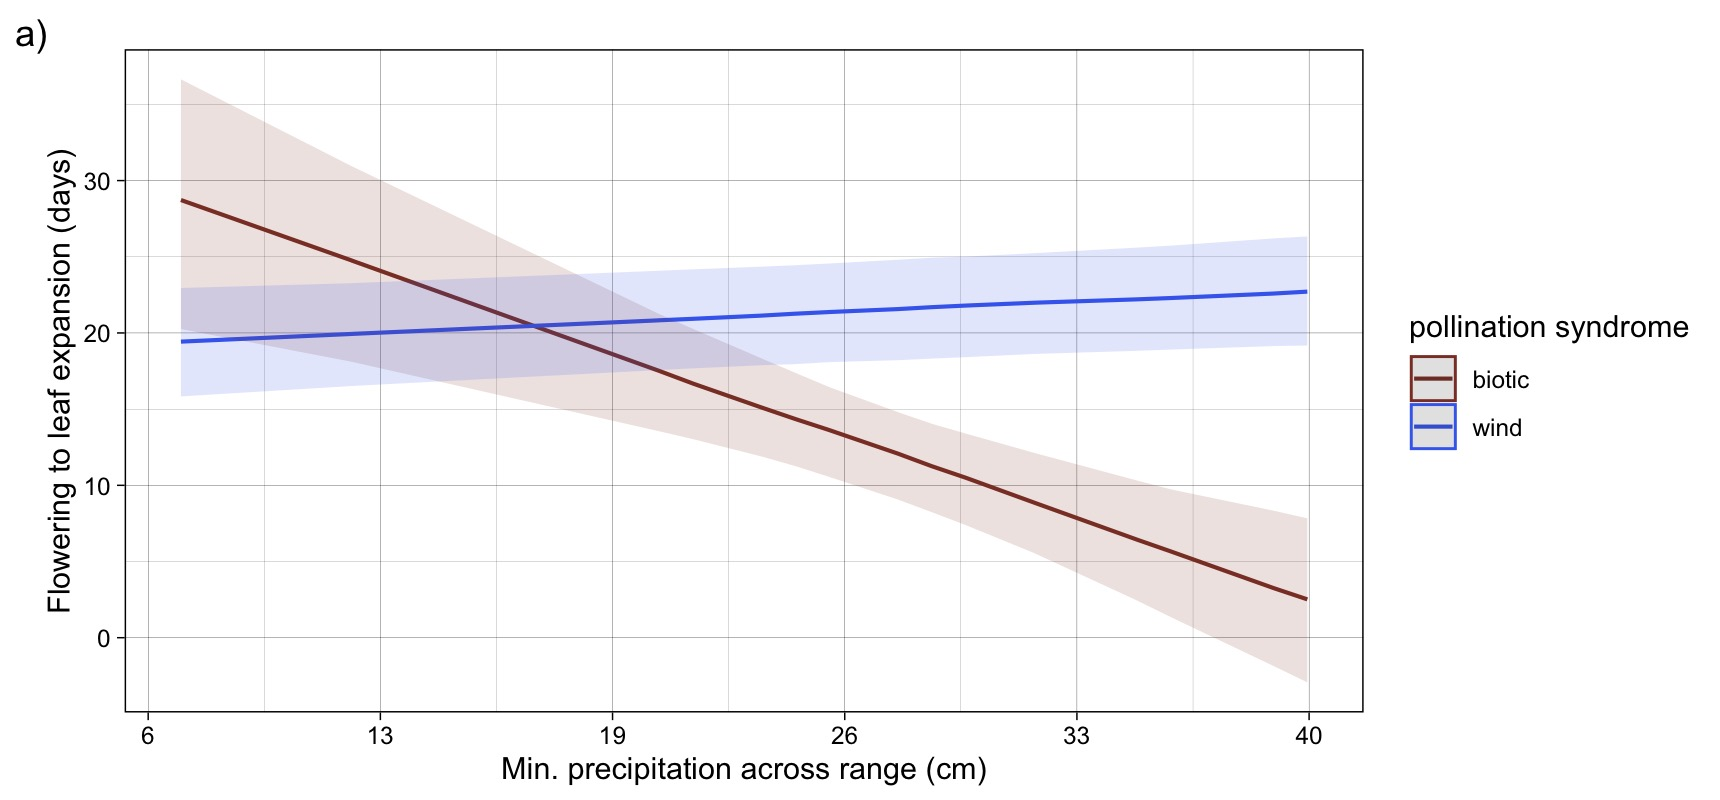
\includegraphics[width=\textwidth]{..//HarvardForest/apcs.jpeg}
           \caption{\textbf{The quantitative flower-leaf sequence (FLS) model suggests that water dynamics may be a driver of hysteranthy in biotically-pollinated but not in wind-pollinated taxa.} Here we show model-predicted differences in FLS as a function the minimum precipitation a across a species' range for a two generic species with contrasting pollination syndromes. These model projections are conditioned on long term phenological data from Harvard Forest in Petersham, MA \citep{OKeefe2015} and reflect a fixed flowering time in early May (approximately the overall long-term average in the community) for both functional types. These systematic differences in drivers of FLSs could reflect greater differences in the bio-geographic histories of the wind and biotically-pollinated taxa of temperate forest communities.}
        \label{fig:apcs}
    \end{figure}


    
\end{document}
